% \chapter{Multi-task learning with Machine Translation}

% \section{POS Tagging}
% By introducing linguistic information to the model, we hypothesize that the original model was not able to extract this information from raw text, and explicitly feed the model with such information will improve it. However, in the unfortunate event that the translation model has already captured the information of POS tags, it might be helpful to use these attention layers to do POS tagging.

\chapter{Interpreting Self-Attention as Parse}
\label{multitask}

In this chapter, we would like to suggest another set of approaches in a multi-task fashion.
Our proposed approaches attempt to jointly parse the source sentence and translate simultaneously by leveraging the self-attention mechanism in the encoder of the \transformer. \cref{multitask-dep} describes the model that is able to parse the source dependency tree and translate. To examine the real benefit of dependency syntax, we let the model to parse a simple sentence structure instead in \cref{multitask-diagonal}.

\section{Self-Attention as Dependency Parse}
\label{multitask-dep}

Before presenting our proposal in \cref{multitask-dep-parsing}, we would like to briefly introduce a neural dependency parsing model which is our main source of inspiration in \cref{multitask-dep-dozat}.

\subsection{Dependency Parser as Head Selection}
\label{multitask-dep-dozat}

The graph-based dependency parsers, which were discussed in \cref{the-ling-dep-parse}, strive to ensure a complete tree structure both during training and inference.
Yet another solution is simpler, which first learns to select the head token of the current token, i.e. head selection, independently.
After the head selection process, a post-editing process handles the output to hereustically remove any existing cycle to form a proper tree.
This approach has proven its effectiveness with the neural network model proposed by \cite{dozat:biaffine:2017}.

The model, illustrated in \cref{fig:biaffine-parser}, utilizes two different LSTMs to learn the representation $h^{(arc-dep)}_i$ and $h^{(arc-head)}_i$ for each input $x_i$ independently. This input $x_i$ is a concatenation of the word embedding and POS embedding at position $i$ in the input sentence.
After that, an operation named \textit{biaffine attention} is employed to produce $S_{ij}$ which is the probability that token $i$ is the head of token $j$:

\[ S_{ij} = biaf(h^{(arc-head)}_i, h^{(arc-dep)}_j) \] where function $biaf$ is a biaffine transformation. All the $S_{ij}$ values form a matrix $S$ which must be column-normalized.
It is then compared against the gold parse tree, encoded as an adjacency matrix (\cref{fig:deptree-vs-matrix}).

In the context of neural network, the concept of biaffine transformation can be defined, among the commonly used linear transformation and bilinear transformation, as follows:

\paragraph{Linear transformation} is a function $f$ of one variable $x$ ($n$-dimensional), which can be written as 

$$f(x)=x^\intercal W$$

where $W$ is the parameter of the transformation.

\paragraph{Bilinear transformation} is a function $f$ of two variables $x_1$ and $x_2$ ($n_1$-dimensional and $n_2$-dimensional, respectively), which can be written as $$f(x_1, x_2)=x_1^\intercal W x_2$$

where $W$ is the parameter of the transformation. For any fixed $x_1$, $f(x_1, x_2)$ is linear in $x_2$ and for any fixed $x_2$, $f(x_1, x_2)$ is linear in $x_1$.

\paragraph{Biaffine transformation} is a function $f$ of two variables $x_1$ and $x_2$ (with dimension of $n_1$ and $n_2$, respectively), which can be written as $$f(x_1, x_2) = x_1^\intercal W_1 x_2 + (x_1\oplus x_2)^\intercal W_2 + b,$$ where $x_1 \oplus x_2 $ is the vector concatenation resulting in an $(n_1+n_2)$-dimensional vector. $W_1, W_2$ and $b$ are parameters with the dimensions of $n_1\times n_2$, $n_1+n_2$ and $1$, in that order.

\begin{figure}[t]
    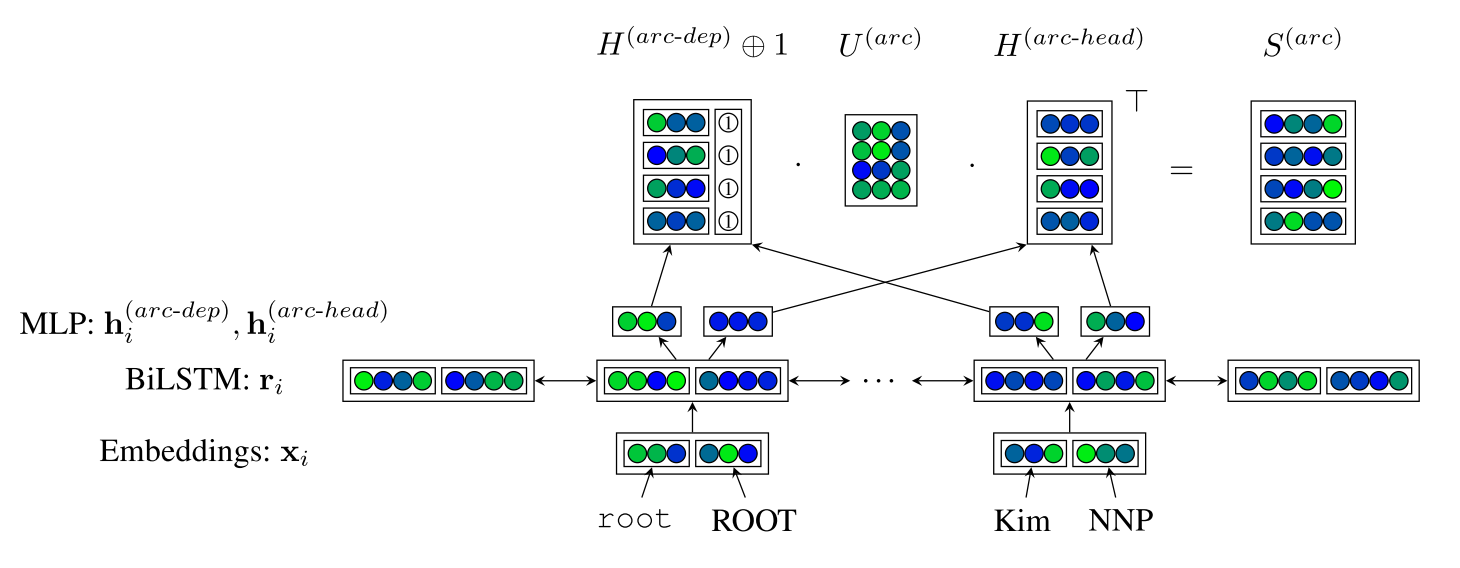
\includegraphics[width=\textwidth]{img/biaffine-parser.png}
    \caption{Neural dependency parser with deep biaffine attention (adapted from \cite{dozat:biaffine:2017})}
    \label{fig:biaffine-parser}
\end{figure}

\begin{figure}[t]
    \begin{minipage}[b]{0.50\linewidth}
        \centering
        \begin{dependency}[text only label]
            \begin{deptext}
            I \& shot \& an \& elephant \& in \& my \& pajamas \\
            \end{deptext}
            \depedge{2}{1}{}
            \depedge{2}{4}{}
            \depedge{4}{3}{}
            \depedge{4}{5}{}
            \depedge{5}{7}{}
            \depedge{7}{6}{}
        \end{dependency}
    % \rule{6cm}{6cm} %to simulate an actual figure
    \end{minipage}%
    \begin{minipage}[b]{0.50\linewidth}
        \centering
            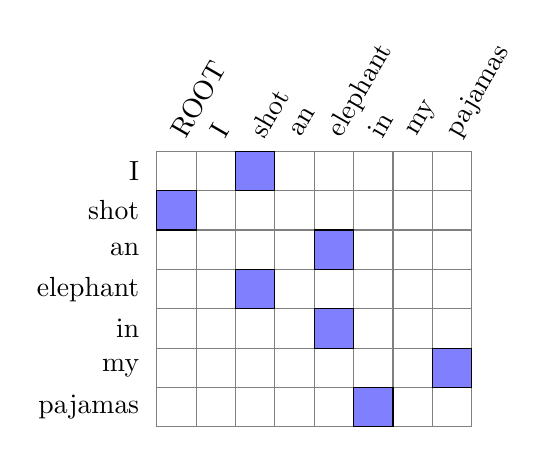
\begin{tikzpicture}[scale=0.5]
                \draw[step=1cm,draw=gray] (0,0) grid (8,7);
                
                \foreach \f [count=\y] in {I, shot, an, elephant, in, my, pajamas} {
                    \node[left] at (-.2,7.5-\y) {{\raggedleft \f }};
                }
                
                \foreach \e [count=\x] in {ROOT, I, shot, an, elephant, in, my, pajamas} {
                    \node[rotate=60,right] at (\x-.6,7.2) {{\raggedright \e}};
                }
                
                % draw word alignment
                \foreach \x [count=\y] in {2, 0, 4, 2, 4, 7, 5} {
                    \draw[fill=blue!50] (\x,7-\y) rectangle +(1,1);
                }
            \end{tikzpicture}
    \end{minipage}
    \caption{A dependency tree and its representation as an adjacency matrix (the columns represent the heads, the rows are dependents).}
    \label{fig:deptree-vs-matrix}
\end{figure}

\subsection{Parsing from Transformer's Self-Attention Weights}
\label{multitask-dep-parsing}

The construction of the $S$ matrix above is very similar to the matrix of self-attention weights $a_{ij}$ in the \transformer model.
From this similarity, we speculate that the self-attentive architecture of \transformer NMT may have the capacity to learn dependency parsing and we only need to promote a little the particular linguistic dependencies captured in a treebank. Hence, we could attempt to simulate this parsing model with the self-attention layer in the \transformer model.

\begin{figure}[t]
    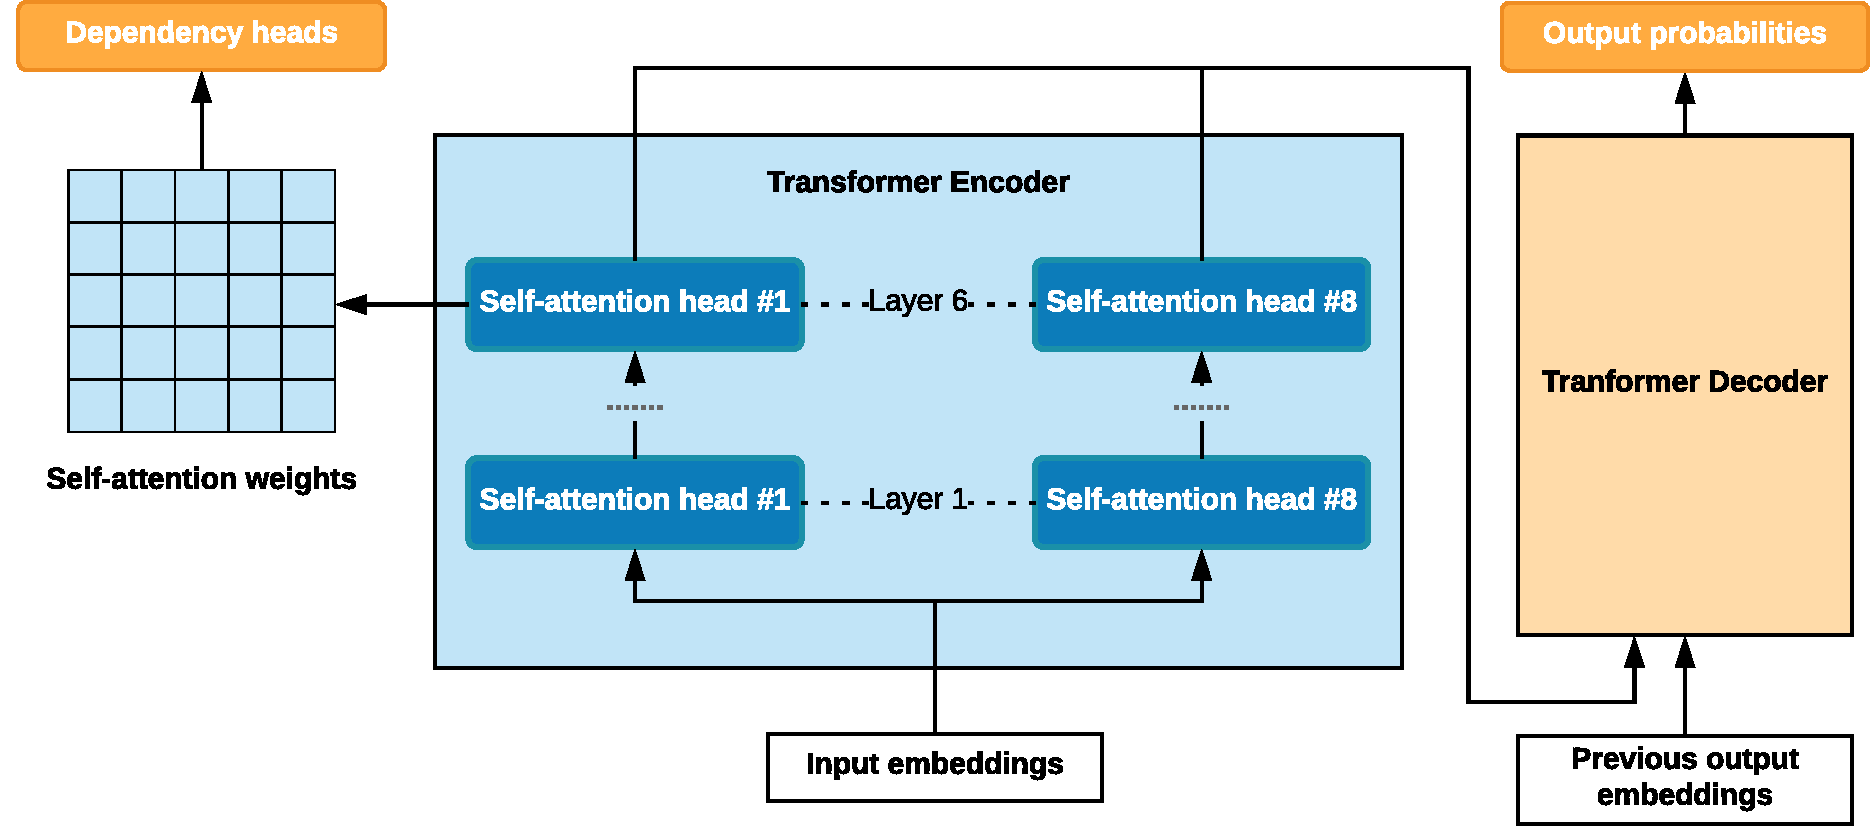
\includegraphics[width=\textwidth]{img/Joint_Translation_DepParse}
    \caption{Joint dependency parsing and translation model (\DepParse and \DiagonalParse).}
    \label{fig:joint_trans_depparse}
\end{figure}

\cref{fig:joint_trans_depparse} illustrates our joint model \DepParse. The translation
part is kept unchanged. The only difference is that we reuse one of the
self-attention heads in the \transformer encoder and reinterpret it as if it was
the dependency matrix $S_{ij}$.
The training objective is combined and
maximizes both the translation quality in terms of cross-entropy of the
candidate translation and the unlabeled attachment score (UAS) of the proposed
heads against the golden parse.\footnote{It should be noted that the dependency
parses we use are actually automatic, produced by
\perscite{mcdonald:pereira:ribarov:hajic:2005} parser incorporated in the Treex
platform, formerly known as TectoMT \parcite{tectomt:popel:2010};
\url{http://ufal.mff.cuni.cz/treex}.}

The particular choice of the head which will serve as the dependency parser is
arbitrary. Put differently, we constrain the \transformer model to use one of its
heads to follow the given syntactic structure of the source sentence. It would be also
possible to use the deep-syntactic parse of the sentence (the
tectogrammatical layer as defined for the Prague Dependency Treebank,
\inparcite{pdt20:2006}); we leave that for future work.

\section{Self-Attention as Diagonal Parse}
\label{multitask-diagonal}

We also would like to conduct an experiment with a simpler sentence structure, which we call the diagonal parse. In a diagonal parse, the dependency head of a token is simply the previous token (\cref{fig:monotree-vs-matrix}).

Our model for the joint diagonal parsing and translation (\DiagonalParse) is identical to the \DepParse model, which has been described in \cref{fig:joint_trans_depparse}. We only need to use the diagonal matrices during training, instead of the dependency matrices.

The main goal of this method is to examine whether or not the dependency structure really helps or any syntactic structure can be beneficial, even a very simple one like this diagonal matrix. 

\begin{figure}[t]
    \begin{minipage}[b]{0.50\linewidth}
        \centering
        \begin{dependency}[text only label]
            \begin{deptext}
            I \& shot \& an \& elephant \& in \& my \& pajamas \\
            \end{deptext}
            \depedge{1}{2}{}
            \depedge{2}{3}{}
            \depedge{3}{4}{}
            \depedge{4}{5}{}
            \depedge{5}{6}{}
            \depedge{6}{7}{}
        \end{dependency}
    % \rule{6cm}{6cm} %to simulate an actual figure
    \end{minipage}%
    \begin{minipage}[b]{0.50\linewidth}
        \centering
            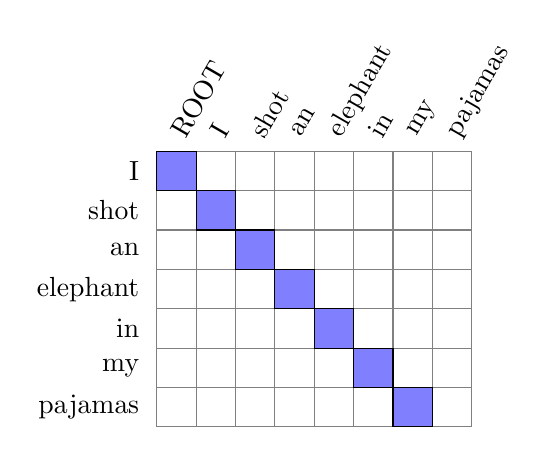
\begin{tikzpicture}[scale=0.5]
                \draw[step=1cm,draw=gray] (0,0) grid (8,7);
                
                \foreach \f [count=\y] in {I, shot, an, elephant, in, my, pajamas} {
                    \node[left] at (-.2,7.5-\y) {{\raggedleft \f }};
                }
                
                \foreach \e [count=\x] in {ROOT, I, shot, an, elephant, in, my, pajamas} {
                    \node[rotate=60,right] at (\x-.6,7.2) {{\raggedright \e}};
                }
                
                % draw word alignment
                \foreach \x [count=\y] in {0, 1, 2, 3, 4, 5, 6} {
                    \draw[fill=blue!50] (\x,7-\y) rectangle +(1,1);
                }
            \end{tikzpicture}
    \end{minipage}
    \caption{An example of the diagonal parse and its diagonal matrix (the columns represent the heads, the rows are dependents).}
    \label{fig:monotree-vs-matrix}
\end{figure}
